\documentclass[10pt]{book}
\usepackage{gvv-book}
\usepackage{gvv}
\usepackage[sectionbib,authoryear]{natbib}% for name-date citation comment the below line
\usepackage{setspace}
\setstretch{1.0}
%\usepackage[sectionbib,numbers]{natbib}% for numbered citation comment the above line
%%********************************************************************%%
%%       How many levels of section head would you like numbered?     %%
%% 0= no section numbers, 1= section, 2= section, 3= subsection %%
\setcounter{secnumdepth}{3}
%%********************************************************************%%
%%**********************************************************************%%
%%     How many levels of section head would you like to appear in the  %%
%%				Table of Contents?			%%
%% 0= chapter, 1= section, 2= section, 3= subsection titles.	%%
\setcounter{tocdepth}{2}
%%**********************************************************************%%
%\includeonly{ch01}
\makeindex
\let\cleardoublepage\clearpage
\begin{document}
\frontmatter
%%%%%%%%%%%%%%%%%%%%%%%%%%%%%%%%%%%%%%%%%%%%%%%%%%%%%%%%%%%%%%%%
\booktitle{Geometry}
\subtitle{Through Algebra}
\AuAff{Errala Paulsonashish}
%\halftitlepage
\titlepage
\tableofcontents
%\listoffigures %optional
%\listoftables  %optional
%% or Contributor Page for edited books
%% before \tableofcontents
%%%%%%%%%%%%%%%%%%%%%%%%%%%%%%%%%%%%%%%%%%%%%%%%%%%%%%%%%%%%%%%%
\setcounter{page}{0}
\begin{introduction}
This book shows how to solve problems in geometry using trigonometry and coordinate geometry. 
\end{introduction}
\mainmatter
\chapter{Triangle}
Consider a triangle with vertices
		\begin{align}
			\label{eq:tri-pts}
			\vec{A} = \myvec{-5 \\ -4},\,
			\vec{B} = \myvec{3 \\ -3},\,
			\vec{C} = \myvec{4 \\ 0}
		\end{align}
\section{Perpendicular Bisector}
\begin{enumerate}[label=\thesection.\arabic*.,ref=\thesection.\theenumi]
\numberwithin{equation}{enumi}
%%\begin{enumerate}[label=\thesection.\arabic*.,ref=\thesection.\theenumi]
\numberwithin{equation}{enumi}

%Question 1.4.1:
\item The equation of the perpendicular bisector of $\vec{BC}$ is
\begin{align}
\label{eq:tri-perp-bisect}
\myvec{\vec{x}-\frac{\vec{B}+\vec{C}}{2}}\brak{\vec{B}-\vec{C}}^{\top} = 0
\end{align}
Substitute numerical values and find the equations of the perpendicular bisectors of $\vec{AB}, \vec{BC}$ and $\vec{CA}$.\\
\solution
\begin{enumerate}
\item  Equation for the perpendicular bisector of $\vec{BC}$ :
\begin{align}
    \myvec{\vec{x}-\frac{\vec{B}+\vec{C}}{2}}\brak{\vec{B}-\vec{C}}^{\top} = 0 \\
    \vec{x}\brak{\vec{B} - \vec{C}}^{\top}= \myvec{\frac{\vec{B}+\vec{C}}{2}}\brak{\vec{B}-\vec{C}}^{\top}
\end{align}
On substituting the values,
\begin{align}
    \vec{\frac{\vec{B}+\vec{C}}{2}} &= \myvec{\frac{7}{2} \\ \frac{-3}{2}} \\
    \vec{B}-\vec{C} &= \myvec{-1\\ -3} \\
    \brak{\vec{B}-\vec{C}}^{\top} &= \myvec{-1 & -3}
\end{align}
solving using matrix multiplication
\begin{align}
\brak{\vec{B}-\vec{C}}^{\top}\brak{\frac{\vec{B}+\vec{C}}{2}}&=0\\
\brak{\vec{B}-\vec{C}}^{\top}\brak{\frac{\vec{B}+\vec{C}}{2}}&=\myvec{-1 & -3}\myvec{\frac{7}{2} \\ \frac{-3}{2}}\\
&= \frac{-7}{2} + \frac{9}{2} \\
& =1
\end{align}
Therefore equation for perpendicular bisector of $\vec{BC}$ is
\begin{align}
    \myvec{-1 & -3}\vec{x}&= 1
\end{align}
\item Similarly the equation for the perpendicular bisector of $\vec{AB}$ :
\begin{align}
    \brak{\vec{x}-\frac{\vec{A}+\vec{B}}{2}}\brak{\vec{A}-\vec{B}}^{\top} = 0 \\
    \vec{x}\brak{\vec{A} - \vec{B}}^{\top}= \myvec{\frac{\vec{A}+\vec{B}}{2}}\brak{\vec{A}-\vec{B}}^{\top}
\end{align}
On substituting the values,
\begin{align}
\vec{\frac{\vec{A}+\vec{B}}{2}} &= \myvec{-1 \\ -\frac{-7}{2}} \\
\vec{A}-\vec{B} &= \myvec{-8 \\ -1} \\
\brak{\vec{A}-\vec{B}}^{\top} &= \myvec{-8 & -1}
\end{align}
solving using matrix multiplication yields
\begin{align}
\brak{\vec{A}-\vec{B}}^{\top}\brak{\frac{\vec{A}+\vec{B}}{2}}&=0 \\
\brak{\vec{A}-\vec{B}}^{\top}\brak{\frac{\vec{A}+\vec{B}}{2}}&=\myvec{-8 & -1}\myvec{-1 \\ \frac{-7}{2}}\\
&= \frac{23}{2}
\end{align}
Therefore equation for perpendicular bisector of $\vec{AB}$ is
\begin{align}
    \myvec{-8 & -1}\vec{x}&= \frac{23}{2}
\end{align}
  \item Similarly the equation for the perpendicular bisector of $\vec{CA}$ :
\begin{align}
    \brak{\vec{x}-\frac{\vec{C}+\vec{A}}{2}}\brak{\vec{C}-\vec{A}}^{\top} = 0 \\
    \vec{x}\brak{\vec{C} - \vec{A}}^{\top}= \myvec{\frac{\vec{C}+\vec{A}}{2}}\brak{\vec{C}-\vec{A}}^{\top}
\end{align}
On substituting the values,
\begin{align}
\vec{\frac{\vec{C}+\vec{A}}{2}} &= \myvec{\frac{-1}{2} \\ -2} \\
\vec{C}-\vec{A} &= \myvec{9 \\ 4} \\
\brak{\vec{C}-\vec{A}}^{\top} &= \myvec{9 & 4}
\end{align}
solving using matrix multiplication
\begin{align}
\brak{\vec{C}-\vec{A}}^{\top}\brak{\frac{\vec{C}+\vec{A}}{2}}&=0 \\
\brak{\vec{C}-\vec{A}}^{\top}\brak{\frac{\vec{C}+\vec{A}}{2}}&=\myvec{9 & 4}\myvec{\frac{-1}{2} \\ -2}
&= \frac{-25}{2}
\end{align}
Therefore equation for perpendicular bisector of $\vec{CA}$ is
\begin{align}
    \myvec{9 & 4}\vec{x}&= \frac{-25}{2}
\end{align}
\end{enumerate}

\begin{figure}[H]
\centering
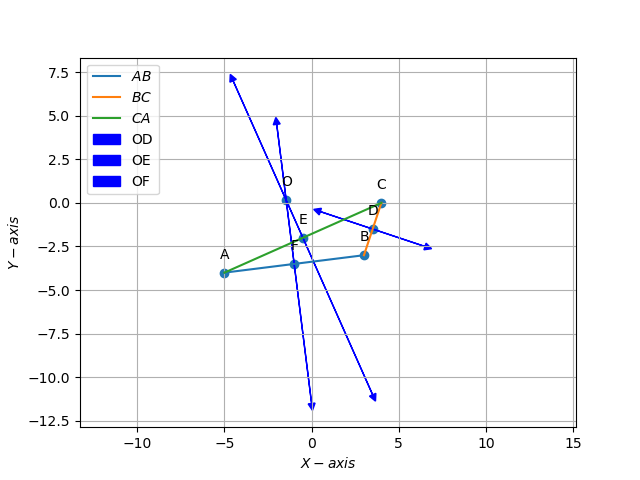
\includegraphics[width=\columnwidth]{figs/perpendicular_bisectors.png}
\caption{Plot of the perpendicular bisectors}
\label{fig:figure1}
\end{figure}


%Question 1.4.2:
\item Find the intersection $\vec{O}$ of the perpendicular bisectors of $\vec{AB}$ and $\vec{AC}$.\\
\solution \\
Given,
\begin{align}
\vec{A}=\myvec{-5 \\ -4},\,
\vec{B}=\myvec{3\\-3},\,
	\vec{C}=\myvec{4\\0},\,
\end{align}

Vector equation of perpendicular bisector of $\vec{A}-\vec{B}$ is
\begin{align}
 (\vec{A}-\vec{B})^\top  \brak{ \vec{x} - \frac{\vec{A}+\vec{B}}{2}} = 0
\end{align}
where,
\begin{align}
\vec{A}+\vec{B}&=\myvec{-2\\ -7}\\
\vec{A}-\vec{B} &= \myvec{-5\\-4}-\myvec{3\\-3}\\
&=\myvec{-8\\-1}\\
\implies (\vec{A}-\vec{B})^\top &= \myvec{-8 &-1}
\end{align}
$\therefore $ The vector equation of $\vec{O}-\vec{F}$ is
\begin{align}
\myvec{-8 & -1} \brak{\vec{x}-\frac{1}{2}\myvec{-2\\7}} &=0 \\
\implies \myvec{-8&-1}\vec{x}&=\frac{1}{2}\brak{\myvec{-8 & -1}\myvec{-2\\-7}}
\end{align}
Performing matrix multiplication yields
\begin{align}
\myvec{-8 & -1}\vec{x}&=\frac{23}{2}
\label{eq:vec-OF}
\end{align}
Similarly vector equation of perpendicular bisector of $\vec{A}-\vec{C}$ is
\begin{align}
\brak{\vec{A}-\vec{C}}^\top\brak{\vec{x} - \frac{\vec{A}+\vec{C}}{2}}=0
\end{align}
where,
\begin{align}
\vec{A}+\vec{C}&=\myvec{-5\\-4}+\myvec{4\\0}\\
&=\myvec{-1\\-4}\\
\vec{A}-\vec{C} &= \myvec{-5\\-4}-\myvec{4\\0}\\
&=\myvec{-9\\-4}\\
\implies (\vec{A}-\vec{C})^\top &= \myvec{-9 &-4}
\end{align}
$\therefore $ The vector equation of $\vec{O}-\vec{E}$ is
\begin{align}
\myvec{-9&-4}\brak{ \vec{x}-\frac{1}{2}\myvec{-1\\-4}}&=0\\
\implies \myvec{-9&-4}\vec{x}&=\frac{1}{2}\brak{\myvec{-9&-4}\myvec{-1\\-4}}
\end{align}
Performing matrix multiplication yields
\begin{align}
\myvec{-9&-4}\vec{x}&=\frac{25}{2}
\label{eq:vec-OE}
\end{align}
Thus, solving equations \eqref{eq:vec-OF} and \eqref{eq:vec-OE} :
\begin{align}
\myvec{-8 & -1& \frac{23}{2} \\ -9 & -4 & \frac{25}{2}} &\xleftrightarrow[]{R_1 \leftarrow \frac{-R_1}{8}} \myvec{1 & \frac{1}{8} & -\frac{23}{16} \\ -9 & -4 & \frac{25}{2}}\\
&\xleftrightarrow[]{R_2 \leftarrow R_2+9R_1}
\myvec{1 & \frac{1}{8} & -\frac{23}{16} \\ 0 & -\frac{23}{8} & -\frac{7}{16}}\\ 
&\xleftrightarrow[]{R_2\leftarrow -\frac{8R_2}{23}} \myvec{1 & \frac{1}{8} & -\frac{23}{16} \\ 0 & 1 & \frac{7}{46}}\\
&\xleftrightarrow[]{R_1\leftarrow R_1 - \frac{R_2}{8}}
 \myvec{1 & 0 & -\frac{67}{46} \\ 0 & 1 & \frac{7}{46}}
\end{align}
Therefore, the point of intersection of perpendicular bisectors of $\vec{A}-\vec{B}$ and $\vec{A}-\vec{C}$ is 
\begin{align}
    \vec{O} = \myvec{-\frac{67}{46}\\ \frac{7}{46}}
    \label{eq:tri-O-bisecter}.
\end{align}

\begin{figure}[H]
\centering
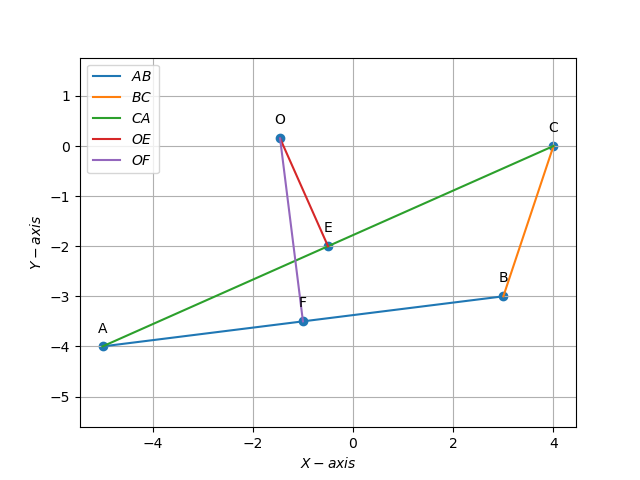
\includegraphics[width=\columnwidth]{figs/OE_OF.png}
\caption{$\vec{O}-\vec{E}$ and $\vec{O}-\vec{F}$ are perpendicular bisectors of $\vec{A}-\vec{C}$ and $\vec{A}-\vec{B}$ respectively}
\label{fig:Figure_2}
\end{figure}

 %Question 1.4.3:
\item Verify that $\vec{O}$ satisfies
\eqref{eq:tri-perp-bisect}.
$\vec{O}$ is known as the circumcentre.\\
 \solution\\
 From the equation \eqref{eq:tri-O-bisecter}. we get,
 \begin{align}
\vec{O}=\myvec{-\frac{67}{46}\\ \frac{7}{46}} \\
\brak{\vec{x}-\frac{\vec{B}+\vec{C}}{2}}\brak{\vec{B}-\vec{C}}^{\top} &= 0
\end{align}
when substitute value in the above equation we get,
\begin{align}
	&=\brak{\vec{O}-\frac{\vec{B}+\vec{C}}{2}}\brak{\vec{B}-\vec{C}}^{\top}\\
	&=\brak{\myvec{-\frac{67}{46}\\ \frac{7}{46}}- \frac{1}{2}\myvec{7\\-3}} \myvec{-1 &-3}\\
	&=\myvec{-\frac{114}{23}\\ \frac{38}{23}}\myvec{-1 &-3}\\
	&=0
\end{align}
It is hence proved that $\vec{O}$ satisfies the equation \eqref{eq:tri-perp-bisect}
\begin{figure}[H]
\centering
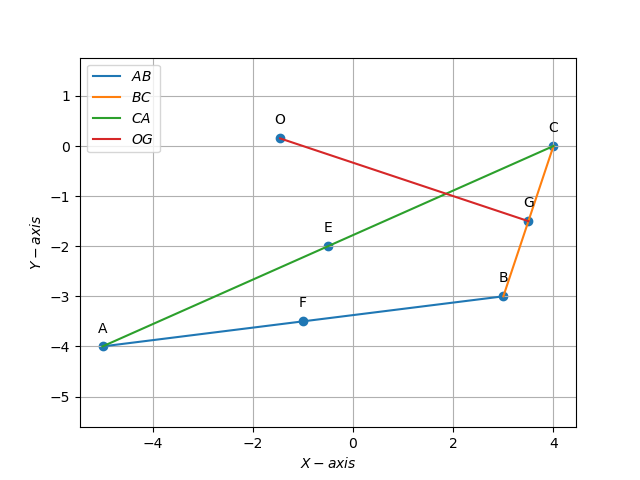
\includegraphics[width=\columnwidth]{figs/O_satisfy.png}
\caption{Circumcenter plotted using python}
\label{fig:Circumcenter to BC}
\end{figure}

 %Question 1.4.4:  
\item Verify that 
\begin{align}
\vec{OA} = \vec{OB} = \vec{OC} 
\end{align} 
\solution \\
Given \begin{align}
\vec{A} &= \myvec{-5\\-4}\\
\vec{B} &= \myvec{3\\-3}\\
\vec{C} &= \myvec{4\\0}
\end{align}
From equation \eqref{eq:tri-O-bisecter} :
\begin{align}
\vec{O} &= \myvec{-\frac{67}{46} \\ \frac{7}{46}}\\
 &= \myvec{-1.45652\\0.15217}
\end{align}
\begin{enumerate}
\item Solving of $\vec{OA}$ :
\begin{align}
\vec{OA}&= \sqrt{(\vec{O}-\vec{A})^{\top}(\vec{O}-\vec{A})}\\
&= \sqrt{\myvec{\frac{163}{46} & \frac{191}{46}} \myvec{\frac{163}{46}\\ \frac{191}{46}}}\\
 &= \sqrt{\frac{63050}{2116}}\\
 &= \frac{\sqrt{63050}}{46}
 \label{eq:tri-OA}
\end{align}
\item Solving of $\vec{OB}$ :
\begin{align}
\vec{OB}&= \sqrt{(\vec{O}-\vec{B})^{\top}(\vec{O}-\vec{B})}\\
 &= \sqrt{\myvec{\frac{-205}{46} & \frac{145}{46}} \myvec{\frac{-205}{46}\\ \frac{145}{46}}}\\
 &= \sqrt{\frac{63050}{2116}}\\
 &= \frac{\sqrt{63050}}{46}
  \label{eq:tri-OB}
\end{align}
\item Solving of $\vec{OC}$ :
\begin{align}
\vec{OC} &= \sqrt{(\vec{O}-\vec{C})^{\top}(\vec{O}-\vec{C})}\\
 &= \sqrt{\myvec{\frac{-251}{46} & \frac{7}{46}}  \myvec{\frac{-251}{46}\\ \frac{7}{46}}}\\
 &= \sqrt{\frac{63050}{2116}}\\
 &= \frac{\sqrt{63050}}{46}
  \label{eq:tri-OC}
\end{align}
\end{enumerate}
From above equations   \eqref{eq:tri-OA} ,\eqref{eq:tri-OB} and \eqref{eq:tri-OC} :
\begin{align}
\vec{OA} = \vec{OB} = \vec{OC}
\end{align}
Hence verified.

%Question 1.4.5:
\item Draw the circle with centre at $\vec{O}$ and radius 
\begin{align}
\vec{R} = \vec{OA}
\end{align}
This is known as the {\em circumradius}. \\
\solution
Given
\begin{align}
\vec{A} &= \myvec{-5\\-4}\\
\vec{B} &= \myvec{3\\-3}\\
\vec{C} &= \myvec{4\\0}
\end{align}
From \eqref{eq:tri-O-bisecter}, the circumcentre is
\begin{align}
\vec{O} = \myvec{\frac{-67}{46}\\ \frac{7}{46}}
\end{align}
Now we will calculate the radius,
\begin{align}
      \vec{R} &= \vec{OA}\\
        &= \norm{\vec{A} - \vec{O}}\\
        &= \norm{\myvec{-5\\-4} - \myvec{\frac{-67}{46}\\ \frac{7}{46}}}\\
        &= \norm{\myvec{\frac{-163}{46}\\ \frac{-191}{46}}}\\
        &=\sqrt{\myvec{\frac{-163}{46} & \frac{-191}{46}}\myvec{\frac{-163}{46}\\ \frac{-191}{46}}} \\
        &= \sqrt{\frac{63050}{2116}} \\
        &= \frac{\sqrt{63050}}{46}
\end{align}
see \figref{fig:circumcircle with centre O}
\begin{figure}[H]
\centering
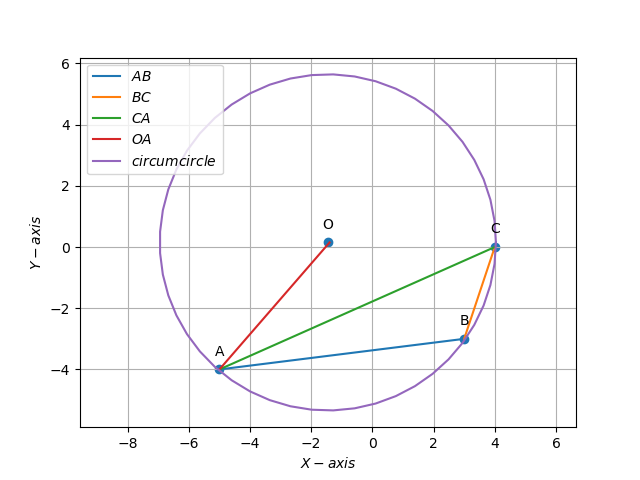
\includegraphics[width=\columnwidth]{figs/circumradius_o.png}
\caption{circumcircle of Triangle ABC with centre O}
\label{fig:circumcircle with centre O}	
\end{figure}

 %Question 1.4.6:
\item Verify that 
\begin{align}
\angle BOC = 2\angle BAC.
\end{align}\\
 \solution
\begin{enumerate}
\item To find  the value of $\angle{BOC}$ :
\begin{align}
\vec{B}-\vec{O}
          &=\myvec{\frac{205}{46}\\\frac{-145}{46}} \\
\vec{C}-\vec{O}
         & =\myvec{\frac{251}{46}\\\frac{-7}{46}}
	  \\
\implies \brak{\vec{B}-\vec{O}}^{\top}\brak{\vec{C}-\vec{O}}&=\frac{26235}{1058}\\
        &= 24.79678\\
	\implies \norm{\vec{B}-\vec{O}}&= \frac{\sqrt{63050}}{46} \\
	\norm{\vec{C}-\vec{O}} &= \frac{\sqrt{63050}}{46}
\end{align}
Thus,
\begin{align}
\cos{BOC}&=\frac{\brak{\vec{B}-\vec{O}}^{\top}\brak{\vec{C}-\vec{O}}}{\norm{\vec{B}-\vec{O}}\norm{\vec{C}-\vec{O}}}
=0.83219\\
\implies\angle{BOC}&=\cos^{-1}\brak{0.83219}\\
&=33.6756\degree
\label{eq:1}
\end{align}
\item To find  the value of $\angle{BAC}$ :
\begin{align}
\vec{B}-\vec{A}&=\myvec{8\\1} \\
\vec{C}-\vec{A}&=\myvec{9\\4}\\
\implies \brak{\vec{B}-\vec{A}}^{\top}\brak{\vec{C}-\vec{A}}&=76\\
\norm{\vec{B}-\vec{A}}&= \sqrt{65}\\
\norm{\vec{C}-\vec{A}}= \sqrt{97}
\end{align}
Thus,
\begin{align}
\cos{BAC}&=\frac{\brak{\vec{B}-\vec{A}}^{\top}\brak{\vec{C}-\vec{A}}}{\norm{\vec{B}-\vec{A}}\norm{\vec{C}-\vec{A}}}
=0.95713\\
\implies\angle{BAC}&=\cos^{-1}\brak{0.95713}\\
&=16.8375\degree 
\label{eq:2}  \\
2\times\angle{BAC} &= 33.675\degree
\end{align}
From \eqref{eq:1} and \eqref{eq:2},
\begin{align}
2\times\angle{BAC}
= \angle{BOC}
\end{align}
Hence Verified.
\begin{figure}[H]
\centering
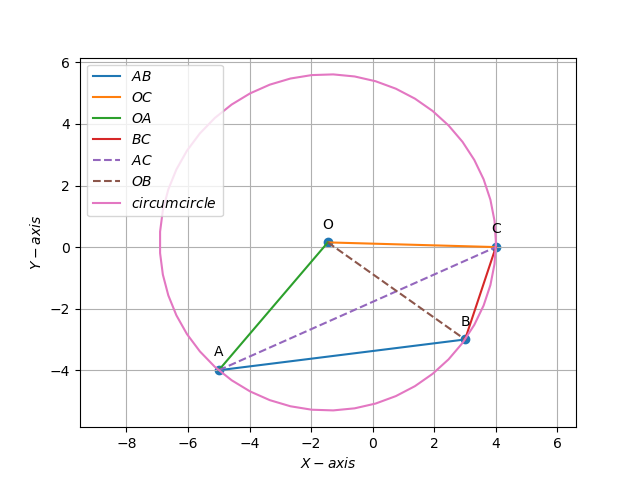
\includegraphics[width=\columnwidth]{figs/Boc_2Bac.png}
	\caption{$\angle{BOC}$ and $\angle{BAC}$}
\label{fig:BOC is 2BAC}
\end{figure}
\end{enumerate}

%Question 1.4.7:
\item Let 
\begin{align}
\vec{P} = \myvec{\cos \theta & -\sin \theta \\ \sin \theta & \cos \theta}
\end{align}
Find $\theta$ if 
\begin{align}
\vec{C}-\vec{O}=\vec{P}\brak{\vec{A}-\vec{O}}
\end{align}
\solution
\begin{align}
    \vec{C}-\vec{O}
          & =\myvec{-4\\\frac{-3}{4}}\\
\vec{A}-\vec{O}
         & =\myvec{-3\\\frac{-11}{4}}\\
\vec{P} &= \myvec{\cos \theta & -\sin \theta \\ \sin \theta & \cos \theta} \\
   \vec{C}-\vec{O}&=\vec{P}\brak{\vec{A}-\vec{O}} \label{eq:1.4.7.6}
\end{align}
 Now from \eqref{eq:1.4.7.6}
 \begin{align}
 \myvec{\frac{251}{46} \\\frac{-7}{46}}&= \myvec{\cos \theta & -\sin \theta \\ \sin \theta & \cos \theta} \myvec{\frac{-163}{46}\\\frac{-191}{46}}    
 \end{align}
solving using matrix multiplication,we get
\begin{align}
    \myvec{\frac{251}{46}\\\frac{-7}{46}}&=\myvec{ \frac{-163}{46}\cos\theta + \frac{191}{46}\sin\theta \\ \frac{-163}{46}\sin\theta + \frac{-191}{46}\cos\theta}
\end{align}
Comparing on Both sides ,we get
\begin{align}
     \frac{-163}{46}\cos\theta + \frac{191}{46}\sin\theta  &= \frac{251}{46}
     \label{eq:1.4.7.9}\\
 \frac{-163}{46}\sin\theta + \frac{-191}{46}\cos\theta &= \frac{-7}{46}
     \label{eq:1.4.7.10}
\end{align}
On solving equations \eqref{eq:1.4.7.9}  and \eqref{eq:1.4.7.10}
\begin{align}
    \cos\theta&= 0.80365\\
    \sin\theta&= 0.59423 \\
    \theta &=\cos^{-1}\brak{0.80365} \\
            &= 36.55\\
    \therefore \theta = 36.55\degree
\end{align}
All codes for this section are available at
\begin{lstlisting}
	geometry/Triangle/perp_Bisector/codes/Allperp_bisectors.py
\end{lstlisting}
\end{enumerate}
\end{document}
